\documentclass{../../../latex/boi2014-lt}

\usepackage{enumitem}
\usepackage{todonotes}
\usepackage{wrapfig}

\renewcommand{\OlympiadDayNum}{2}
\renewcommand{\TaskCode}{portals}
\renewcommand{\TaskName}{Portals}

\newcommand{\param}[1]{{\tt #1}}
\newcommand{\method}[1]{{\tt #1}}
\newcommand{\constant}[1]{{\tt #1}}

\begin{document}
    There is a cake placed inside of a labyrinth and you desperately want
    to eat it. You have a map of the labyrinth, which is
    a grid of $R$ rows and $C$ columns.
    Each grid cell contains one of the following characters:
    \begin{description}[itemindent=1pt]
    	\item[\constant{\#}] (number sign) which denotes a wall,
        \item[\constant{.}] (dot) which denotes an open square,
        \item[\constant{S}] (uppercase letter s) which denotes your current position,
        \item[\constant{C}] (uppercase letter c) which denotes the position of the cake.
    \end{description}
    You may only walk on the open squares. Additionally, the rectangular
    area depicted on the map is surrounded by walls from the outside
    with no open spaces.

    In order to reach the cake faster you have acquired a portal gun from
    Aperture Science\texttrademark{}, which operates as follows.
    At any time it can fire a portal in one of the four directions
    \emph{up}, \emph{left}, \emph{down} and \emph{right}.
    When a portal is fired in some direction, it will fly in that direction
    until it reaches the first wall. When this happens, a portal
    will be spawned on the side of that wall that faces you.

    At most two portals can exist at any given time. If two portals
    are already placed in the labyrinth, then one of them (selected
    by you) will be removed immediately upon using the portal gun
    again. Firing a portal at a wall where there is already a portal
    placed will replace that portal (there may be at most one portal
    per side of wall).
    Note that there may be multiple portals placed
    on different sides of same wall.
    \todo{Did I get this note right?}

    Once two portals are placed on the map you can use them to
    teleport yourself. When standing next to one of the portals,
    you can walk into it and end up at the square next to the other
    portal. Doing this takes as much time as moving between two
    adjacent squares.

    You may assume that firing portals does not take time and moving
    between two squares (or teleporting through portals) takes one unit
    of time.

    \Task
    Given the map of the labyrinth together with your starting location
    and the location of the cake, calculate the minimum possible time needed
    for you to reach the cake.

    \Implementation
    You need to implement the function \method{get\_cake(R, C, M)}
    which takes the following parameters:
    \begin{itemize}
        \item \param{R} --- the number of rows in the map $R$,
        \item \param{C} --- the number of columns in the map $C$,
        \item \param{M} --- a two--dimensional array, where
            \param{M}$[i][j]$ ($0 \le i < R$, $0 \le j < C$) is the cell in
             the $i$--th row and $j$--th column of the map.
    \end{itemize}

    It is guaranteed that characters \constant{S} and \constant{C} each appear
    exactly once in the map, and that it is always possible to reach the cake
    from your starting location.

    The function has to return the minimum time that is needed to reach the cake
    from the starting position.

    \Example
    \begin{wrapfigure}[5]{r}{3cm}
        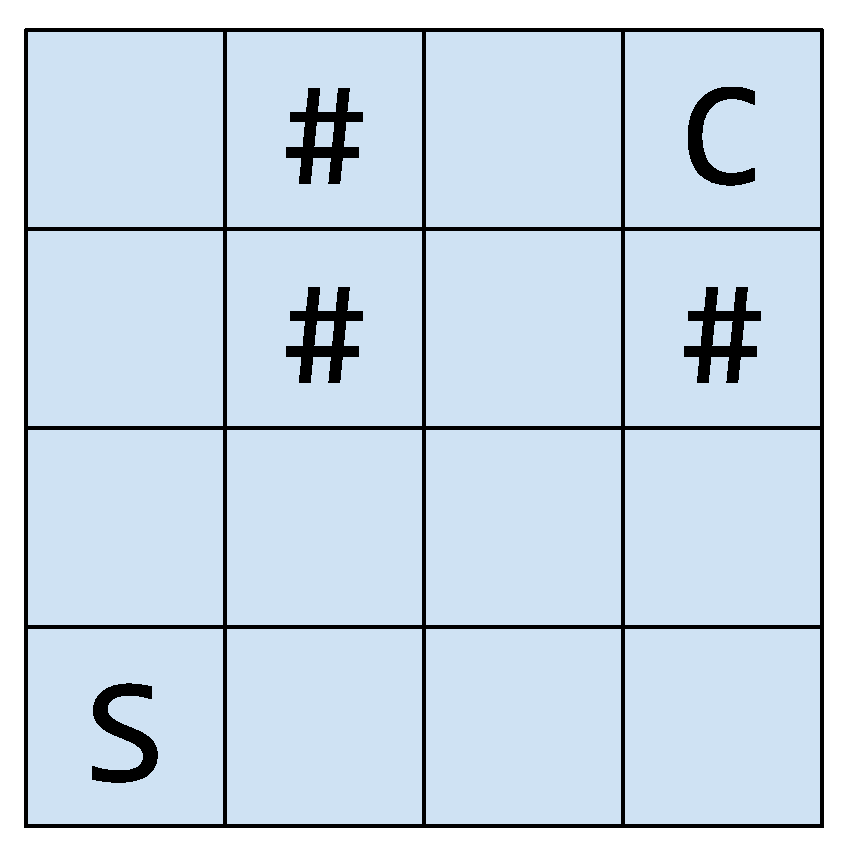
\includegraphics[width=3cm]{fig-example}
    \end{wrapfigure}
    Let us consider the example illustrated on the right.
    One quickest sequence of moves is as follows:

    \begin{enumerate}
        \item move right
        \item move right, shoot one portal up, and one portal down
        \item move through the bottom portal --- you will appear at 
            the location $row = 0, column = 2$
        \item move one square right and reach the cake.
    \end{enumerate}

    This takes time $4$ and no quicker way is possible. Therefore
    function \method{get\_cake} should return~\constant{4}.

    \Scoring

    \begin{description}
        \item[Subtask 1 (25 points):] $0 \le R \le 2, 0 \le C \le 2$.
        \item[Subtask 2 (25 points):] $0 \le R \le 10, 0 \le C \le 10$.
        \item[Subtask 3 (25 points):] $0 \le R \le 100, 0 \le C \le 100$.
        \item[Subtask 4 (25 points):] $0 \le R \le 1000, 0 \le C \le 1000$.
    \end{description}

    \Constraints

    \begin{description}
        \item[Time limit:] 1 s.
        \item[Memory limit:] 256 MB.
    \end{description}

    \todo{Need to add info about graders.}
\end{document}
